% Chapter 1

\chapter{Introducción general} % Main chapter title

\label{Chapter1} % For referencing the chapter elsewhere, use \ref{Chapter1}
\label{IntroGeneral}

En este capítulo se presenta el área en la que se enmarca el trabajo, el contexto y la motivación que le dieron origen, una revisión del estado del arte en la clasificación automática de sonidos de auscultación y los objetivos y el alcance del proyecto.

%----------------------------------------------------------------------------------------

\section{La auscultación cardiopulmonar}
\label{sec:auscultacion}

La auscultación es la técnica de exploración clínica que consiste en escuchar los sonidos generados en el interior del cuerpo, principalmente los del corazón y los pulmones. Desde que René Laënnec inventó el estetoscopio en 1816 y lo utilizó para vincular los sonidos torácicos con los hallazgos de autopsia \citep{roguin2006laennec}, la auscultación se convirtió en uno de los pilares del examen físico. Su vigencia se explica por tres características: es no invasiva, tiene un costo muy bajo y brinda información inmediata en el lugar de atención.

Los sonidos cardíacos normales se originan principalmente en el cierre de las válvulas y se perciben como dos golpes breves por ciclo, conocidos como primer y segundo ruido (S1 y S2). Distintas alteraciones modifican este patrón. Los soplos son sonidos producidos por el flujo turbulento de la sangre y se asocian, por ejemplo, a valvulopatías o a cardiopatías congénitas. También pueden aparecer ruidos adicionales, como el tercer y el cuarto ruido (S3 y S4), o irregularidades del ritmo. En el caso de los pulmones, el flujo de aire durante la respiración produce los ruidos respiratorios normales. Sobre ellos pueden superponerse sonidos adventicios, como los crepitantes, que son eventos discontinuos y de muy corta duración, y las sibilancias, que son sonidos continuos de carácter musical. Ambos se asocian a patologías como la neumonía, la fibrosis pulmonar, el asma o la enfermedad pulmonar obstructiva crónica \citep{bohadana2014fundamentals}.

La principal limitación de la auscultación es su subjetividad: la interpretación de los sonidos depende en gran medida del entrenamiento y de la experiencia del profesional. En un estudio multicéntrico con más de 450 médicos en formación de medicina interna y medicina familiar, los participantes identificaron correctamente, en promedio, alrededor del 20\,\% de los eventos cardíacos que se les presentaron, sin mejoras significativas a medida que avanzaban en la residencia \citep{mangione1997cardiac}.

La aparición del estetoscopio electrónico modificó este escenario. Este dispositivo convierte la señal acústica en una señal eléctrica que puede amplificarse, filtrarse, almacenarse y transmitirse \citep{leng2015electronic}. Contar con la auscultación como una señal digital la vuelve compatible con las técnicas de procesamiento de señales y de aprendizaje automático. En particular, las redes neuronales profundas pueden aprender directamente, a partir de representaciones tiempo-frecuencia como el espectrograma, los patrones acústicos que caracterizan a cada patología. En la figura \ref{fig:ejemplosAuscultacion} se muestran ejemplos de estas representaciones para sonidos cardíacos y pulmonares, normales y patológicos. Este trabajo se sitúa en ese cruce entre la auscultación digital y la inteligencia artificial.

\begin{figure}[htbp]
	\centering
	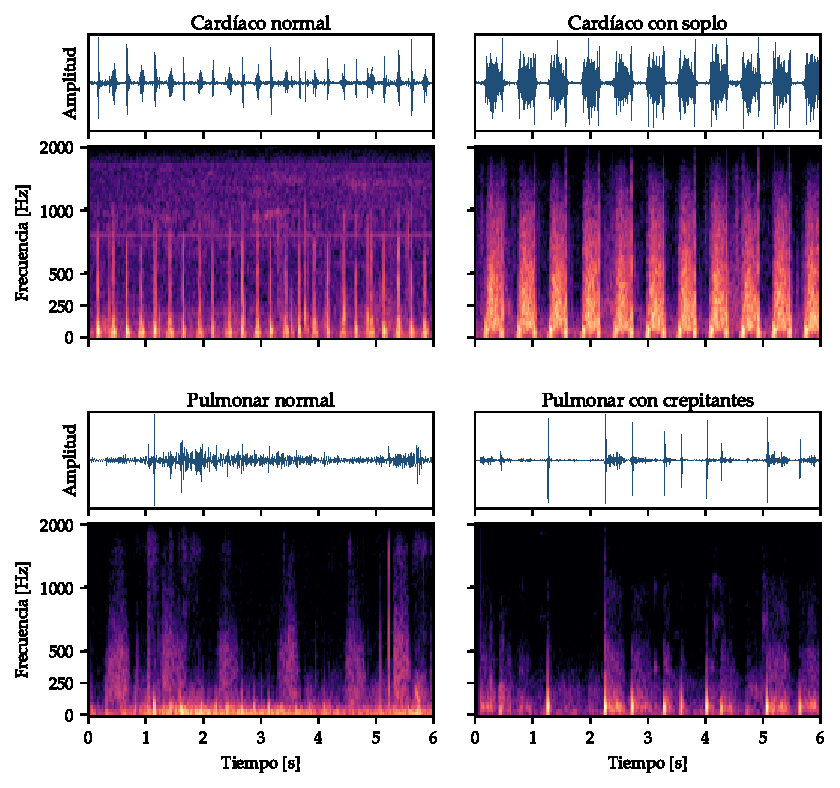
\includegraphics[width=\textwidth]{./Figures/ejemplos_auscultacion.pdf}
	\caption{Forma de onda y espectrograma en escala Mel de cuatro grabaciones de auscultación: sonido cardíaco normal, sonido cardíaco con soplo, sonido pulmonar normal y sonido pulmonar con crepitantes.}
	\label{fig:ejemplosAuscultacion}
\end{figure}

%----------------------------------------------------------------------------------------

\section{Contexto y motivación}
\label{sec:motivacion}

Las enfermedades cardiovasculares y respiratorias se encuentran entre las principales causas de muerte y de discapacidad en el mundo. Según la Organización Mundial de la Salud, en 2019 las enfermedades cardiovasculares causaron alrededor de 17,9 millones de muertes, el 32\,\% del total mundial, y más de tres cuartas partes de ellas ocurrieron en países de ingresos bajos y medios \citep{who2021cvd}. Por su parte, en 2017 se estimaba que unas 545 millones de personas vivían con alguna enfermedad respiratoria crónica, que en conjunto constituían la tercera causa de muerte a nivel mundial \citep{gbd2020chronic}. En ambos grupos de enfermedades, la detección temprana resulta determinante para el pronóstico del paciente y para reducir los costos que la enfermedad avanzada impone al sistema de salud.

El acceso a esa detección temprana no es homogéneo. En América del Sur, los profesionales de la salud se concentran en las capitales y en las grandes ciudades, mientras que las zonas rurales y desatendidas sufren faltantes que afectan de manera directa la disponibilidad de especialistas \citep{paho2026brechas}. En esos contextos, suele ser el médico generalista quien realiza la primera evaluación del paciente con el estetoscopio y quien decide, a partir de lo que escucha, si derivarlo o no a un cardiólogo o a un neumólogo. Como se señaló en la sección \ref{sec:auscultacion}, la precisión de esa evaluación depende fuertemente del entrenamiento del profesional. Un soplo o un crepitante que pasan inadvertidos pueden retrasar el diagnóstico de una enfermedad tratable. A la inversa, una derivación innecesaria consume recursos escasos.

Este escenario motiva el desarrollo de herramientas de apoyo a la decisión clínica basadas en inteligencia artificial. Un sistema capaz de analizar la señal registrada por un estetoscopio digital y de indicar la presencia de hallazgos patológicos ofrecería al médico generalista una segunda opinión objetiva y reproducible, sin reemplazar su criterio. Además, en la práctica clínica el corazón y los pulmones se auscultan durante el mismo examen, por lo que resulta de interés que una misma herramienta pueda analizar ambos tipos de sonido.

El trabajo se desarrolló en el marco de la Carrera de Especialización en Inteligencia Artificial de la Universidad de Buenos Aires, en colaboración con el Centro de Investigación y Desarrollo en Ingeniería Biomédica (CIBIO) de la Universidad Tecnológica Nacional, Facultad Regional Buenos Aires. Sus resultados son de carácter académico y de acceso abierto, para que puedan incorporarse a futuras líneas de investigación clínica del centro. Desde el punto de vista del autor, el proyecto integra su experiencia previa en procesamiento digital de señales y en desarrollos aplicados al ámbito médico con las técnicas de aprendizaje profundo estudiadas durante la especialización.

%----------------------------------------------------------------------------------------

\section{Estado del arte}
\label{sec:estadoArte}

El análisis automático de sonidos de auscultación tuvo un fuerte crecimiento durante la última década, impulsado en buena medida por la publicación de bases de datos abiertas y por desafíos científicos que permitieron comparar algoritmos bajo condiciones comunes. En el dominio cardíaco se destacan el desafío PhysioNet/Computing in Cardiology 2016, orientado a distinguir grabaciones normales de anormales \citep{clifford2016classification}, y el George B. Moody PhysioNet Challenge 2022, centrado en la detección de soplos \citep{reyna2023heart} sobre la base CirCor DigiScope, compuesta por grabaciones de pacientes pediátricos \citep{oliveira2022circor}. En el dominio pulmonar, la referencia principal es la base del desafío ICBHI 2017, con 920 grabaciones de 126 pacientes y anotaciones de crepitantes y sibilancias por ciclo respiratorio \citep{rocha2019open}. Revisiones recientes de ambos dominios muestran que el aprendizaje profundo desplazó a los métodos basados en características diseñadas manualmente \citep{ren2024comprehensive, sfayyih2023review}.

El enfoque predominante consiste en transformar la señal de audio en una representación tiempo-frecuencia, como el espectrograma en escala Mel o los coeficientes cepstrales en frecuencia Mel (MFCC, \textit{Mel-Frequency Cepstral Coefficients}), y procesarla con una red neuronal convolucional (CNN, \textit{Convolutional Neural Network}). En el desafío de 2016, la mejor propuesta combinó un clasificador basado en características con una CNN \citep{potes2016ensemble}, mientras que en el de 2022 el primer puesto en la detección de soplos correspondió a una CNN liviana que recibe el espectrograma Mel junto con datos demográficos del paciente \citep{lu2022lightweight}. En el dominio pulmonar, los trabajos más recientes incorporan transferencia de aprendizaje desde modelos preentrenados sobre grandes volúmenes de imágenes o de audio general. RespireNet adaptó una ResNet-34 preentrenada en ImageNet con técnicas de aumentación específicas para sonidos respiratorios \citep{gairola2021respirenet}, y trabajos posteriores emplearon arquitecturas basadas en \textit{transformers}, como el \textit{Audio Spectrogram Transformer}, combinadas con aprendizaje contrastivo \citep{bae2023patchmix}. La tabla \ref{tab:estadoArte} resume los trabajos más representativos.

\begin{table}[htbp]
	\centering
	\caption[Comparación de trabajos representativos del estado del arte]{Comparación de trabajos representativos en la clasificación automática de sonidos de auscultación. Se informa la métrica principal de cada trabajo sobre su conjunto de prueba; los valores no son directamente comparables entre filas porque difieren las tareas, los datos y los protocolos de partición.}
	\label{tab:estadoArte}
	\small
	\begin{tabular}{>{\raggedright\arraybackslash}p{2.0cm} >{\raggedright\arraybackslash}p{2.3cm} >{\raggedright\arraybackslash}p{2.3cm} >{\raggedright\arraybackslash}p{2.9cm} >{\raggedright\arraybackslash}p{2.1cm}}
		\toprule
		\textbf{Trabajo} & \textbf{Tarea} & \textbf{Datos} & \textbf{Modelo} & \textbf{Resultado} \\
		\midrule
		Potes et al. \citep{potes2016ensemble} & Cardíaco: normal o anormal & PhysioNet/ CinC 2016 & Ensamble de AdaBoost sobre características y CNN & Puntaje 0,860 (1.\textsuperscript{er} puesto) \\
		\addlinespace
		Lu et al. \citep{lu2022lightweight} & Cardíaco: soplo presente, ausente o desconocido & CirCor DigiScope & CNN liviana sobre espectrograma Mel y datos demográficos & Exactitud ponderada 0,780 (1.\textsuperscript{er} puesto) \\
		\addlinespace
		Gairola et al. \citep{gairola2021respirenet} & Pulmonar: 4 clases de sonidos adventicios por ciclo & ICBHI 2017 (partición oficial) & ResNet-34 preentrenada en ImageNet & Puntaje ICBHI 56,2\,\% (Se 40,1\,\%, Sp 72,3\,\%) \\
		\addlinespace
		Bae et al. \citep{bae2023patchmix} & Pulmonar: 4 clases de sonidos adventicios por ciclo & ICBHI 2017 (partición oficial) & \textit{Audio Spectrogram Transformer} con aprendizaje contrastivo & Puntaje ICBHI 62,4\,\% (Se 43,1\,\%, Sp 81,7\,\%) \\
		\addlinespace
		Tariq et al. \citep{tariq2022feature} & Pulmonar y cardíaco, con un modelo para cada dominio & ICBHI 2017 y una base pública de 656 grabaciones cardíacas & Fusión de tres CNN (espectrograma, MFCC y cromagrama) & Exactitud 99,1\,\% (pulmonar) y 97\,\% (cardíaco) \\
		\bottomrule
	\end{tabular}
\end{table}

La comparación entre trabajos debe hacerse con cautela. Cada desafío define su propia métrica: el de 2016 y el ICBHI utilizan el promedio entre sensibilidad (Se) y especificidad (Sp), mientras que el de 2022 emplea una exactitud ponderada que penaliza más los soplos no detectados. Además, la forma de particionar los datos influye fuertemente en los resultados. Sobre la partición oficial del ICBHI, los trabajos de la tabla \ref{tab:estadoArte} obtienen puntajes de entre el 56 y el 62\,\%, con sensibilidades por debajo del 45\,\%. En cambio, algunos trabajos informan exactitudes cercanas al 99\,\% con una partición 80/20 de las grabaciones, sin indicar si las grabaciones de un mismo paciente quedan separadas entre entrenamiento y prueba \citep{tariq2022feature}. Cuando esa separación no se garantiza, el modelo puede aprender características propias de cada paciente o de cada equipo de grabación, y el resultado sobreestima su desempeño ante pacientes nuevos.

Por último, la gran mayoría de los sistemas existentes aborda los sonidos cardíacos y pulmonares como dominios independientes: cada modelo se entrena con una única base de datos y reconoce solo patologías de un órgano. Incluso los trabajos que estudian ambos tipos de sonido, como el de Tariq et al., entrenan y evalúan un modelo distinto para cada dominio \citep{tariq2022feature}. Esta separación contrasta con la práctica clínica, en la que el médico ausculta el corazón y los pulmones durante un mismo examen. Recién en los últimos años aparecieron bases de datos que registran ambos sonidos de forma conjunta, como HLS-CMDS, grabada sobre un maniquí clínico \citep{torabi2025hlscmds}, lo que refleja un interés creciente por el análisis cardiopulmonar integrado. El presente trabajo se enfoca en ese vacío: abordar los sonidos cardíacos y pulmonares dentro de un mismo sistema de clasificación.

%----------------------------------------------------------------------------------------

\section{Objetivos y alcance}
\label{sec:objetivos}

% Pendiente.
